\documentclass[12pt,a4paper]{article}

\usepackage[margin=2.5cm]{geometry}
\usepackage{titlesec}
\usepackage{enumitem}
\usepackage{parskip}
\usepackage{fancyhdr}
\usepackage{hyperref}
\usepackage{xcolor}
\usepackage{array}
\usepackage{booktabs}
\usepackage{graphicx}
\usepackage{tikz}
\usetikzlibrary{positioning, arrows.meta, shapes.geometric}

% Disable word hyphenation at line breaks
\hyphenpenalty=10000
\exhyphenpenalty=10000

% Colours
\definecolor{dsoBlue}{RGB}{0,51,102}
\definecolor{dsoGrey}{RGB}{100,100,100}

% Section formatting
\titleformat{\section}{\Large\bfseries\color{black}}{}{0em}{}[\titlerule]
\titleformat{\subsection}{\large\bfseries\color{black}}{}{0em}{}
\titlespacing*{\section}{0pt}{2em}{1em}
\titlespacing*{\subsection}{0pt}{1.5em}{0.5em}

% Header / footer
\pagestyle{fancy}
\fancyhf{}
\fancyhead[L]{\small\color{dsoGrey}Internship Report}
\fancyhead[R]{\small\color{dsoGrey}DSO National Laboratories}
\fancyfoot[C]{\small\color{dsoGrey}\thepage}
\renewcommand{\headrulewidth}{0.4pt}

\begin{document}

% ============================================================
% COVER / HEADER BLOCK
% ============================================================

\begin{center}
    {\LARGE\bfseries\color{black} Internship Report}
\end{center}

\vspace{1em}

\renewcommand{\arraystretch}{1.8}
\begin{tabular}{|m{5.5cm}|m{9.5cm}|}
\hline
\textbf{\color{black}Name of Intern}          & Eugene Ng Yi Sheng \\
\hline
\textbf{\color{black}Name of DSO Supervisor}  & Shen BingQuan \\
\hline
\textbf{\color{black}Date of Internship}       & 11/05/2026\ \ to\ \ 04/08/2026 \\
\hline
\textbf{\color{black}Division / Department}    & Information \\
\hline
\end{tabular}

\vspace{2em}

% ============================================================
% 1. OVERVIEW
% ============================================================
\section{Overview of Internship Assignment}

My internship was centred on designing, building, and evaluating a \textbf{multi-agent marketplace simulation} that tests how cooperation mechanisms shape the behaviour of self-interested Large Language Model (LLM) agents under adversarial conditions.

\medskip
\noindent\textbf{Research Question:} Can cooperation mechanisms help self-interested LLM agents sustain positive utility under escalating adversarial pressure, and which mechanism designs are most robust to progressive infiltration?

\subsection*{Literature Review}

A growing body of research has examined whether LLM agents can cooperate in structured social dilemmas, and what conditions are required to sustain that cooperation.

\textbf{CoopEval} \cite{coopeval} established a foundational benchmark showing that without any institutional support, all modern LLMs default to defection in repeated social dilemmas. Their study tested several mechanisms including contracting and mediation, finding that mechanisms which structurally alter the payoff matrix, rather than merely providing information, were most effective at inducing cooperation.

\textbf{Corrupted by Reasoning} \cite{corrupted} demonstrated a counterintuitive finding: more capable, reasoning-heavy LLMs become more effective free-riders, not more cooperative. Greater reasoning ability enables agents to identify and exploit loopholes rather than honour the spirit of agreements, suggesting that capability alone does not translate to prosocial behaviour.

\textbf{RepuNet} \cite{repunet} showed that combining reputation systems with dynamic network rewiring and gossip can achieve cooperation rates of 85 to 98\%. However, these results were obtained in relatively benign settings without persistent adversarial actors.

\textbf{The Subtle Art of Defection} \cite{subtleart} found that even a single defector can collapse an otherwise cooperative system within 1 to 7 rounds, highlighting the fragility of cooperation under adversarial pressure and motivating the need for robust institutional safeguards.

Taken together, these works reveal two key gaps. First, most studies do not inject adversarial agents into their simulations, and those that do use fixed adversarial populations rather than escalating pressure over time \cite{repunet}. Second, the experimental environments themselves tend to be fairly simplistic, typically grid-based social dilemmas rather than richer economic settings with production, trade, and spoilage dynamics \cite{coopeval}. Building on these foundations, this project adapts and extends these ideas into a custom marketplace economy where nine mechanisms are compared simultaneously under progressive adversarial injection, allowing direct comparison of enforcement-based, information-based, and insurance-based designs within a unified experimental framework.

\subsection*{The Simulation Environment}

The simulated marketplace consists of 18 LLM agents, each specialising in producing one of three goods (A, B, or C) while needing the other two. This creates mutual dependence and a strong incentive to trade. Each round, agents produce goods, communicate with neighbours, negotiate and execute trades, then consume goods to earn utility. A 20\% per-round spoilage rate penalises hoarding, ensuring that cooperation --- not stockpiling --- is the dominant strategy for a rational agent.

Agents are powered by \textbf{DeepSeek-V3} and reason through each decision using chain-of-thought prompts. Every round, an agent sees its own inventory, utility history, and the outputs of whichever institutional mechanism is active in its condition. The simulation runs for \textbf{200 rounds} per game.

\begin{figure}[h]
\centering
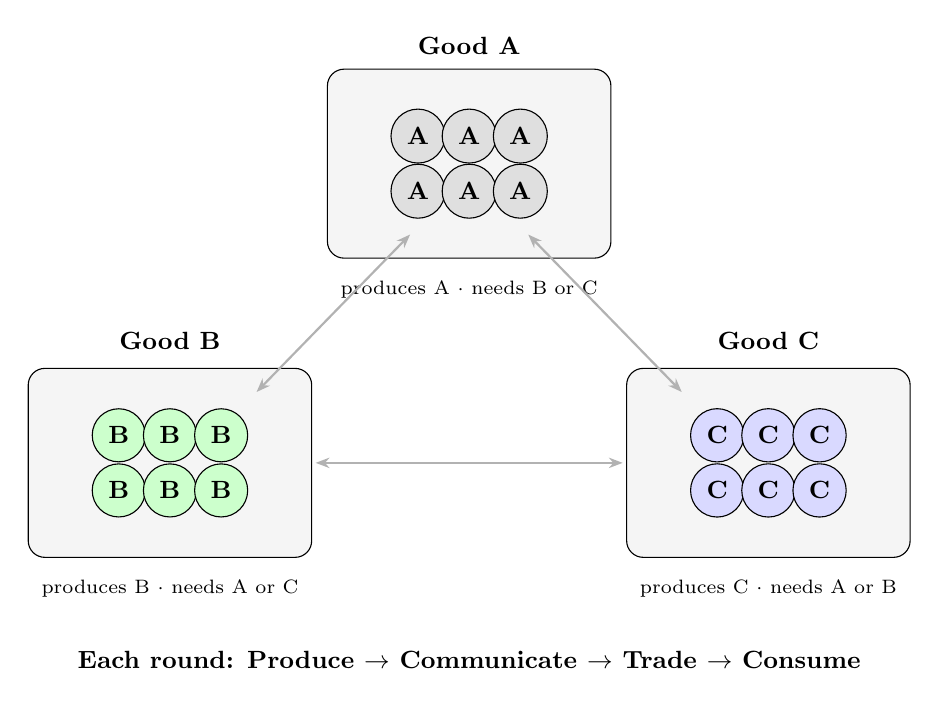
\begin{tikzpicture}[
    groupbox/.style={draw, rounded corners=6pt, fill=gray!8, minimum width=3.6cm, minimum height=2.4cm},
    agentA/.style={draw, circle, fill=gray!25,  minimum size=0.65cm, font=\small\bfseries},
    agentB/.style={draw, circle, fill=green!20, minimum size=0.65cm, font=\small\bfseries},
    agentC/.style={draw, circle, fill=blue!15,  minimum size=0.65cm, font=\small\bfseries},
    biarr/.style={{Stealth[length=5pt]}-{Stealth[length=5pt]}, gray!60, thick}
]

% ---- Group A (top centre) ----
% Label above box
\node[font=\small\bfseries]      at ( 0.0,  5.30) {Good A};
% Box (agents only inside)
\node[groupbox] at (0.0, 3.8) {};
\foreach \x in {-0.65, 0.0, 0.65} { \node[agentA] at (\x, 4.15) {A}; }
\foreach \x in {-0.65, 0.0, 0.65} { \node[agentA] at (\x, 3.45) {A}; }
% Label below box
\node[font=\scriptsize]          at ( 0.0,  2.2) {produces A $\cdot$ needs B or C};

% ---- Group B (bottom left) ----
\node[font=\small\bfseries]      at (-3.8,  1.55) {Good B};
\node[groupbox] at (-3.8, 0.0) {};
\foreach \x in {-4.45, -3.8, -3.15} { \node[agentB] at (\x,  0.35) {B}; }
\foreach \x in {-4.45, -3.8, -3.15} { \node[agentB] at (\x, -0.35) {B}; }
\node[font=\scriptsize]          at (-3.8, -1.6) {produces B $\cdot$ needs A or C};

% ---- Group C (bottom right) ----
\node[font=\small\bfseries]      at ( 3.8,  1.55) {Good C};
\node[groupbox] at ( 3.8, 0.0) {};
\foreach \x in {3.15, 3.8, 4.45} { \node[agentC] at (\x,  0.35) {C}; }
\foreach \x in {3.15, 3.8, 4.45} { \node[agentC] at (\x, -0.35) {C}; }
\node[font=\scriptsize]          at ( 3.8, -1.6) {produces C $\cdot$ needs A or B};

% ---- Trade arrows ----
\draw[biarr] (-0.75, 2.9) -- (-2.7, 0.9);   % A <-> B
\draw[biarr] ( 0.75, 2.9) -- ( 2.7, 0.9);   % A <-> C
\draw[biarr] (-1.95, 0.0) -- ( 1.95, 0.0);  % B <-> C

% ---- Round flow (below all boxes) ----
\node[font=\small\bfseries] at (0, -2.5)
    {Each round: Produce $\rightarrow$ Communicate $\rightarrow$ Trade $\rightarrow$ Consume};

\end{tikzpicture}
\caption{Marketplace structure: three specialised agent groups trade to earn utility. Each group produces one good but needs the other two, creating mutual dependence.}
\label{fig:marketplace}
\end{figure}

\subsection*{Adversarial Stress Testing}

To test whether each mechanism can keep the marketplace functioning (agents still earning positive utility) even as adversarial agents multiply, the simulation uses \textbf{progressive troll injection}: a schedule of deterministic defector agents injected mid-game at rounds 51, 101, and 151, escalating from 0 to 4, then 8, then 16 trolls out of up to 34 total agents (47\% adversarial by the final phase). Trolls always accept trades and always defect --- they take goods without delivering. Crucially, they appear silently; honest agents must discover them through experience rather than announcement.

\subsection*{The Nine Conditions}

The study compares \textbf{nine experimental conditions}, each layering a different institutional mechanism on top of the same base marketplace:

\begin{itemize}
    \item \textbf{B} --- Baseline: no mechanism, pure barter.
    \item \textbf{GR} --- Global Reputation: a system-computed trust score visible to all agents.
    \item \textbf{C} --- Contracting: binding pre-trade agreements with breach penalties.
    \item \textbf{M} --- Mediation: agents may delegate trades to a neutral mediator.
    \item \textbf{G} --- Governance: an omniscient oracle detects defectors and levies fines or suspensions.
    \item \textbf{NR} --- Network Rewiring + Local Reputation: agents sever links to bad actors based on unverified gossip.
    \item \textbf{S} --- Sanctioning: agents spend utility to inflict loss on suspected defectors (3:1 cost ratio).
    \item \textbf{J} --- Judicial: a complaint-driven court where victims file grievances citing a specific trade. The court verifies against ground-truth trade history; guilty verdicts fine the defector and compensate the victim, while frivolous filings incur additional penalties.
    \item \textbf{E} --- Escrow: a shared insurance pool (starting balance: 100 utility) that automatically compensates defection victims. When the pool reaches zero, all agents' accumulated utility resets to zero --- a mutually assured destruction event.
\end{itemize}

\subsection*{Metrics and Objectives}

Two core metrics are tracked, computed over non-troll agents only:

\begin{itemize}
    \item \textbf{Mean utility per round} --- the average per-agent utility gain each round, capturing whether agents are net-positive from trade after production costs.
    \item \textbf{Gini coefficient} --- the inequality of utility distribution across agents, indicating whether gains are broadly shared or concentrated.
\end{itemize}

The primary objective is to determine which institutional mechanisms sustain cooperation most effectively as adversarial pressure escalates, and to understand which design principles --- enforcement, information quality, and collective insurance --- allow agents to continue earning positive utility even when a large fraction of the population is adversarial.



% ============================================================
% 2. APPLICATION TO DSO MISSION
% ============================================================
\section{Application to DSO's Mission and Vision}

DSO's mission is \textit{``to develop technologies and solutions that can provide technological surprises to sharpen the cutting edge of Singapore's national security,''} underpinned by a vision to be \textit{``a wellspring of technological knowledge, a fountain of innovation and an inspiration to the R\&D community.''}

The work undertaken during this internship is directly relevant to this mission in the following ways.

\subsection*{Understanding AI Agent Behaviour Under Adversarial Conditions}

As the use of multi-agent AI systems grows across both commercial and defence domains, ensuring that these systems remain safe and robust against adversarial actors becomes increasingly important. In real-world deployments, it is rarely sufficient to evaluate an AI system only under cooperative or benign conditions. Adversarial actors may infiltrate, manipulate, or free-ride on shared systems, and the question of how quickly a multi-agent system degrades, and whether it can recover, is one that current research has not fully answered.

This project directly addresses that gap by providing a controlled, measurable environment to study how different institutional structures either sustain or fail under escalating adversarial pressure. Rather than testing a single fixed level of adversarial stress, the progressive injection design introduces adversarial agents in waves, allowing us to observe at what threshold each mechanism begins to break down and how sharply it does so. The results can help characterise the resilience profile of each institutional design, distinguishing mechanisms under which agents continue to earn positive utility from those where utility collapses to zero.

This aligns with DSO's mission to develop technologies that sharpen Singapore's national security edge, particularly as AI-driven systems become candidates for deployment in high-stakes operational contexts.

\subsection*{Building Internal Competency in LLM Agent Research}

Beyond the specific findings, the project contributes to DSO's broader research capability in LLM-based agent systems. The simulation framework, including the prompt engineering pipeline, mechanism plugin architecture, and analysis tooling, forms a reusable platform for future experiments on AI cooperation, deception detection, and emergent behaviour in multi-agent settings. This positions the Division to rapidly iterate on new research questions as the LLM landscape evolves, consistent with DSO's vision of being a fountain of innovation in the R\&D community.



% ============================================================
% 3. CHALLENGES
% ============================================================
\section{Challenges Faced During Internship}

The internship began with a wide brief around multi-agent AI cooperation, and the topic was broad enough that it was initially unclear which specific angle would be most productive. To narrow the scope, I read extensively through the existing literature, working through papers on LLM cooperation, social dilemmas, reputation systems, and mechanism design. This process helped me identify what had already been done and where the gaps were. Under the guidance of my supervisor BingQuan, we were able to arrive at a clear direction, ultimately shaping the project towards comparing multiple cooperation mechanisms under adversarial stress in a marketplace setting.

% ============================================================
% 4. LESSONS LEARNT
% ============================================================
\section{Lessons Learnt}

\begin{enumerate}[leftmargin=2em]
    \item \textbf{Taking the initiative to read broadly builds ideas and intuition.} Much of the project's direction came from reading research papers beyond the immediate scope of the assignment. By exploring work on social dilemmas, mechanism design, reputation systems, and adversarial robustness, I was able to draw connections across different fields and generate ideas that would not have emerged from a narrower focus. This taught me that investing time in broad reading, even when the payoff is not immediately obvious, compounds over time and sharpens the quality of the decisions you make later in the project.
    \item \textbf{Iteration is part of the process.} There were many points during the project where early runs produced inconclusive or underwhelming results. Rather than treating these as failures, I learnt to use them as feedback. Each round of iteration, whether it was simplifying the metrics, changing the troll injection approach, or fixing flaws in the mechanism design, brought the experiment closer to producing meaningful insights. The project went through several major redesigns before arriving at its current form, and each one was motivated by what the previous version revealed.
\end{enumerate}

% ============================================================
% 5. POSITIVE EXPERIENCES
% ============================================================
\section{Positive Experiences in DSO}

\begin{enumerate}[leftmargin=2em]
    \item \textbf{A supportive supervisor who trusted me with autonomy.} Going into the project, I had little prior experience with AI agent society simulations. Despite this, BingQuan gave me the space to read up on research papers and do my own exploration rather than prescribing every step. This autonomy was instrumental in helping me develop both the technical depth and the independent thinking needed to shape the project. It also made the work feel genuinely my own, which was a strong motivator throughout the internship.
    \item \textbf{The friendships built along the way.} Beyond the technical work, one of the highlights of the internship was the people. The friends I made during my time at DSO made the experience far more enjoyable, and lunch breaks became something I genuinely looked forward to every day.
\end{enumerate}



% ============================================================
% 6. AREAS TO IMPROVE
% ============================================================
\section{Areas to Improve}

Running large-scale LLM simulations requires significant compute, particularly when each experimental condition involves 200 rounds of multi-agent interaction with API calls to a hosted model. The compute budget available was limited, which meant that experiments had to be planned carefully and some exploratory runs had to be deferred or scaled down. Additionally, compute resources were shared across multiple team members, which occasionally created scheduling conflicts when multiple people needed to run intensive workloads at the same time. That said, we managed to work around this through coordination, taking turns on the shared infrastructure, and prioritising which experiments to run first. A dedicated or ringfenced compute allocation for research-heavy intern projects would help reduce this friction in future.



% ============================================================
% 7. RECOMMENDED CHANGES
% ============================================================
\section{Recommended Changes}

One of the steepest parts of the learning curve was not the technical content but the practice of research itself: how to scope a problem, conduct a literature review efficiently, decide when to pivot, and manage the uncertainty of not knowing whether your experiments will produce conclusive results. A brief onboarding session at the start of the internship, even just one or two hours, covering these topics would help future interns ramp up faster and spend less time feeling lost in the early weeks. This could be as simple as a senior researcher sharing their own workflow and common pitfalls, rather than a formal training programme.



% ============================================================
% 8. EXPECTATIONS
% ============================================================
\section{Whether Initial Expectations Have Been Met}

My initial expectations have not only been met but exceeded. Coming into the internship, my primary hope was to gain a deeper understanding of what research work looks like in practice, beyond what I had been exposed to in a classroom setting. DSO provided exactly the platform for that. I was given a real research problem with genuine uncertainty, access to the tools and compute needed to run large-scale experiments, and a supervisor who guided me without constraining my exploration.

What exceeded my expectations was the degree of ownership I was given over the project. I did not expect to be involved in every stage of the research process, from literature review and problem formulation through to mechanism design, implementation, and analysis. The experience felt less like a supervised exercise and more like genuine research, and that is something I did not anticipate going in.



% ============================================================
% 9. THOUGHTS ABOUT SUPERVISOR
% ============================================================
\section{Thoughts About Your Internship Supervisor}

BingQuan has been a supportive and effective supervisor throughout this internship. As mentioned earlier, he gave me the autonomy to conduct my own research and build the project independently, which was essential for my growth. Rather than dictating what to do at each step, he trusted me to explore the problem space on my own, read broadly, and form my own views before coming to him for discussion. This approach pushed me to take ownership of the work and develop confidence in making design decisions.

At the same time, BingQuan was always available to provide direction during moments where I felt stuck and had exhausted my own ideas. He has a knack for asking the right questions that would reframe the problem and open up new avenues I had not considered.

One area where I lacked experience coming in was the practice of research work itself. Having come from a more application-focused background, I was unfamiliar with how to scope a research project, manage uncertainty in results, and decide when to pivot. I was concerned at times that the project might not produce conclusive findings, but BingQuan was reassuring that even intermediate results carry value and can be meaningfully presented. This perspective helped me stay motivated and not become discouraged when early experiments did not yield clear outcomes. It also taught me that research is inherently iterative, and that negative or ambiguous results still contribute to the overall understanding.

What I appreciated most was BingQuan's ability to think ahead. He would often anticipate future roadblocks in the project well before I encountered them, whether it was a metric that would not scale, a mechanism design that would produce degenerate behaviour, or an experimental setup that would be too costly to run. This kind of foresight saved me significant time and effort, allowing me to course-correct early rather than discover issues after running expensive simulations. It is something I could not have provided on my own given my limited research experience, and it was one of the most valuable aspects of his mentorship.



% ============================================================
% 10. FUTURE CAREER
% ============================================================
\section{Thoughts on Your Future Career}

This internship has strengthened my interest in pursuing a research-oriented career. Before joining DSO, I was interested in AI and data science, but my exposure was largely limited to coursework and project-based applications. Through this internship, I gained firsthand experience in conducting research, from reviewing academic literature and identifying research gaps to designing experiments and analysing results.

Working on multi-agent AI systems has broadened my perspective on artificial intelligence research. Prior to the internship, I primarily viewed AI through the lens of model development and applications. Through this project, I was exposed to broader research questions involving cooperation, incentives, governance mechanisms, and emergent behaviour in complex systems. I found it particularly rewarding to investigate open-ended problems where there may not be a single correct answer, but rather a need for careful experimentation, critical thinking, and evidence-based analysis.

Overall, this internship has reinforced my interest in research and innovation. It has given me a clearer understanding of the type of work I find meaningful and has strengthened my desire to pursue opportunities that involve tackling challenging problems through rigorous investigation. The experience has also increased my appreciation for the role that research organisations such as DSO play in developing advanced technologies and addressing complex real-world challenges. I would be keen to continue contributing to this type of work in the future.



\begin{thebibliography}{9}

\bibitem{coopeval}
Tewolde, E., Zhang, X., Piedrahita, D.G., Conitzer, V., et al. (2026). \textit{CoopEval: Benchmarking cooperation-sustaining mechanisms and LLM agents in social dilemmas}. arXiv:2604.15267.

\bibitem{corrupted}
Piedrahita, D.G., Yang, Y., Sachan, M., Ramponi, G., et al. (2025). \textit{Corrupted by reasoning: Reasoning language models become free-riders in public goods games}. arXiv:2506.23276.

\bibitem{repunet}
Ren, S., Fu, W., Zou, X., Shen, C., Cai, Y., Chu, C., et al. (2025). \textit{Reputation as a Solution to Cooperation Collapse in LLM-based Multi-Agent Systems}. arXiv:2505.05029.

\bibitem{subtleart}
Kulshreshtha, D., Du, W., Jain, R., Doss, S., et al. (2026). \textit{The subtle art of defection: Understanding uncooperative behaviors in LLM based multi-agent systems}. Proceedings of EACL (Industry Track).

\end{thebibliography}

\end{document}
